\subsection{Periodo Requirements and Technology Baseline}
\subsubsection{MPP1 - Schedule variance}

\begin{figure}[H]
	\centering
	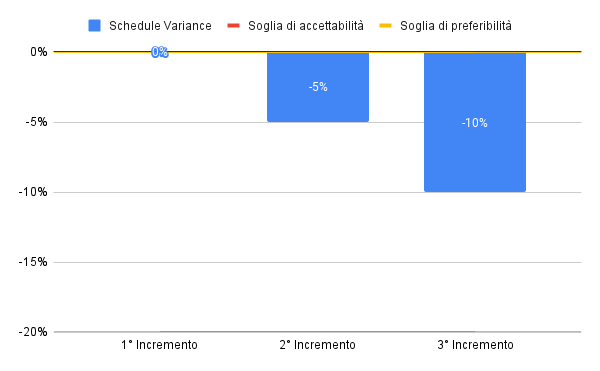
\includegraphics[scale = 0.6]{sezioni/Images/ScheduleVariance.png}
	\caption{MPP1 - Schedule variance}
\end{figure}

\subsubsection{MPP2 - Budget variance}

\begin{figure}[H]
	\centering
	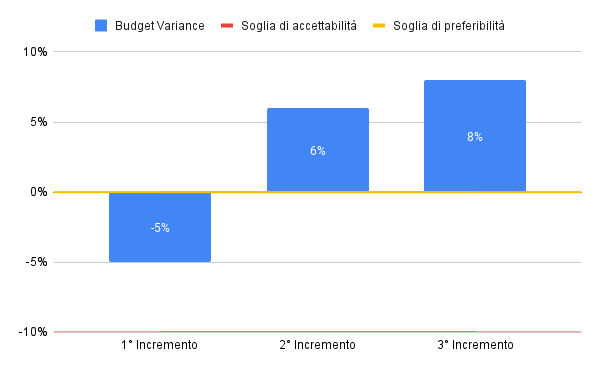
\includegraphics[scale = 0.6]{sezioni/Images/BudgetVariance.png}
	\caption{MPP2 - Budget variance}
\end{figure}

\subsubsection{MPP5 - SPICE capability}

\begin{figure}[H]
	\centering
	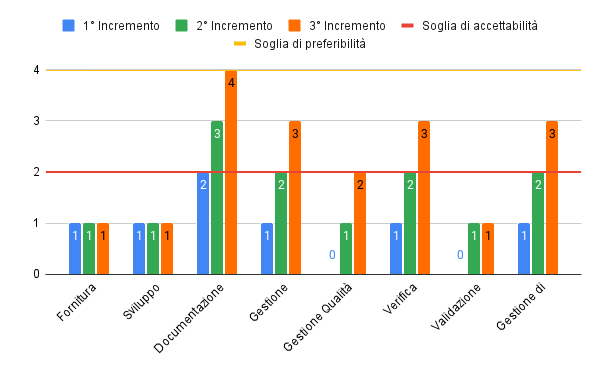
\includegraphics[scale = 0.6]{sezioni/Images/SPICECapability.png}
	\caption{MPP5 - SPICE capability}
\end{figure}

\subsubsection{MPP6 - Requirements Stability Index}

\begin{figure}[H]
	\centering
	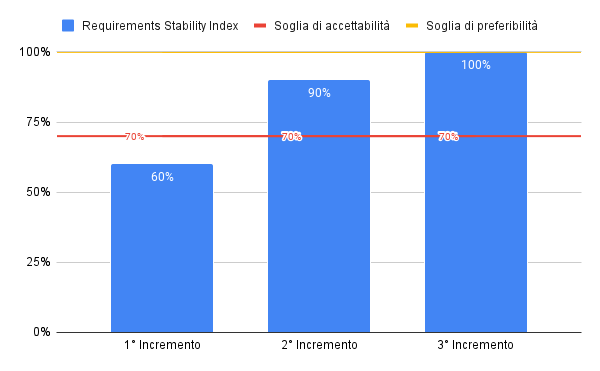
\includegraphics[scale = 0.6]{sezioni/Images/RequirementsStabilityIndex.png}
	\caption{MPP6 - Requirements Stability Index}
\end{figure}

\subsubsection{MPR1 - Indice di Gulpease}

\paragraph{Norme di progetto} \aCapo{}

\begin{figure}[H]
	\centering
	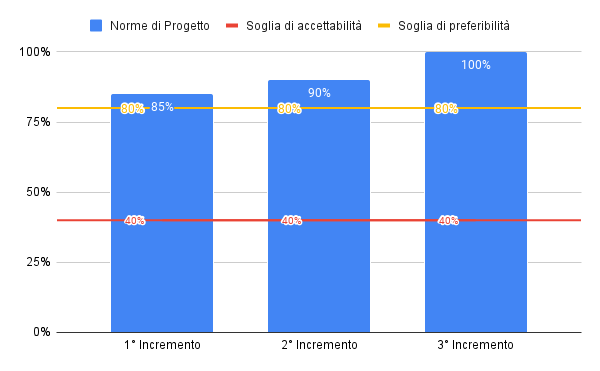
\includegraphics[scale = 0.6]{sezioni/Images/NdP.png}
	\caption{MPR1 - Indice di Gulpease delle norme di progetto}
\end{figure}

\paragraph{Piano di progetto} \textbf{•}

\begin{figure}[H]
	\centering
	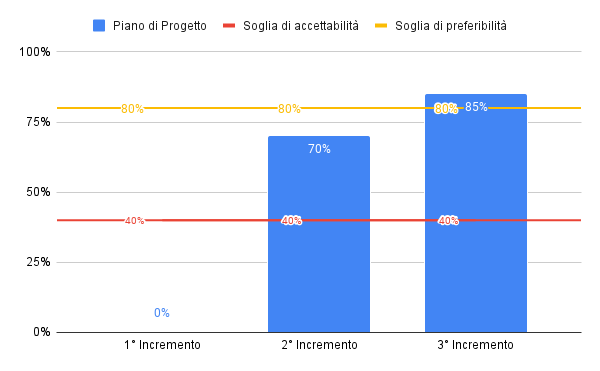
\includegraphics[scale = 0.6]{sezioni/Images/PdP.png}
	\caption{MPR1 - Indice di Gulpease del piano di progetto}
\end{figure}

\paragraph{Piano di qualifica} \aCapo{}

\begin{figure}[H]
	\centering
	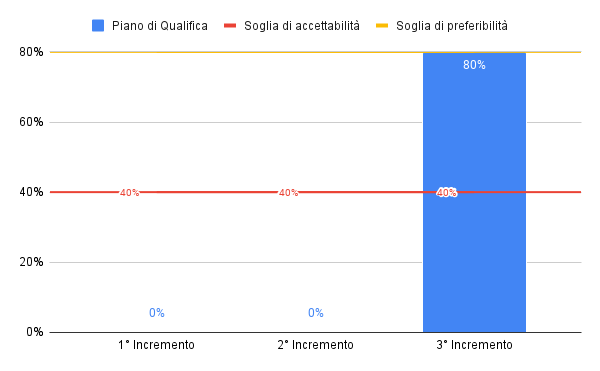
\includegraphics[scale = 0.6]{sezioni/Images/PdQ.png}
	\caption{MPR1 - Indice di Gulpease del piano di qualifica}
\end{figure}

\paragraph{Analisi dei requisiti} \aCapo{}

\begin{figure}[H]
	\centering
	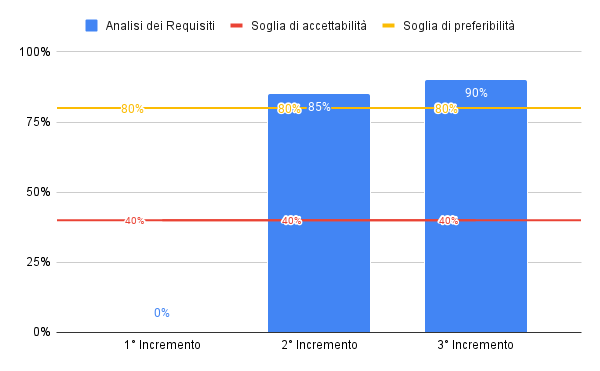
\includegraphics[scale = 0.6]{sezioni/Images/AdR.png}
	\caption{MPR1 - Indice di Gulpease dell'analisi dei requisiti}
\end{figure}

\paragraph{Glossario} \aCapo{}

\begin{figure}[H]
	\centering
	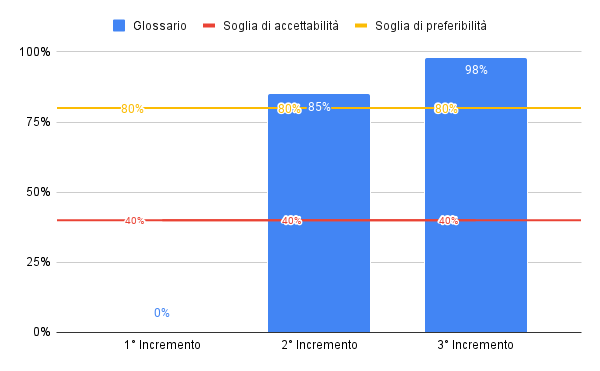
\includegraphics[scale = 0.6]{sezioni/Images/Glossario.png}
	\caption{MPR1 - Indice di Gulpease del glossario}
\end{figure}

\subsection{Product Baseline}
\subsubsection{MPP1 - Schedule variance}

\begin{figure}[H]
	\centering
	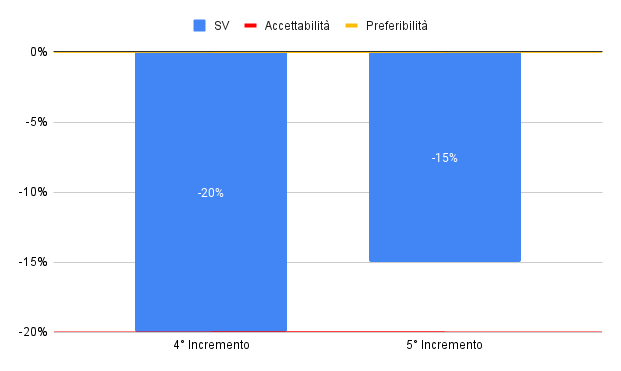
\includegraphics[scale = 0.6]{sezioni/Images/PB/SV.png}
	\caption{MPP1 - Schedule variance}
\end{figure}

\subsubsection{MPP2 - Budget variance}

\begin{figure}[H]
	\centering
	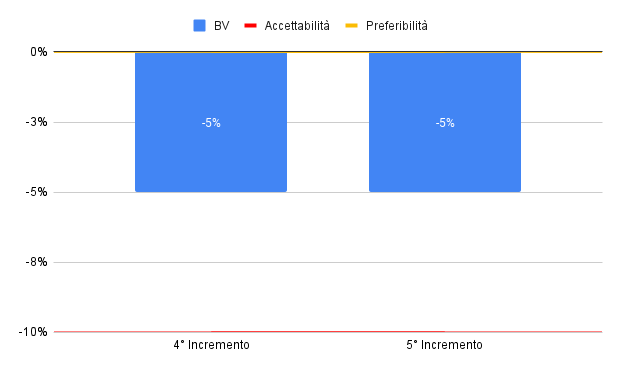
\includegraphics[scale = 0.6]{sezioni/Images/PB/BV.png}
	\caption{MPP2 - Budget variance}
\end{figure}

\subsubsection{MPP5 - SPICE capability}

\begin{figure}[H]
	\centering
	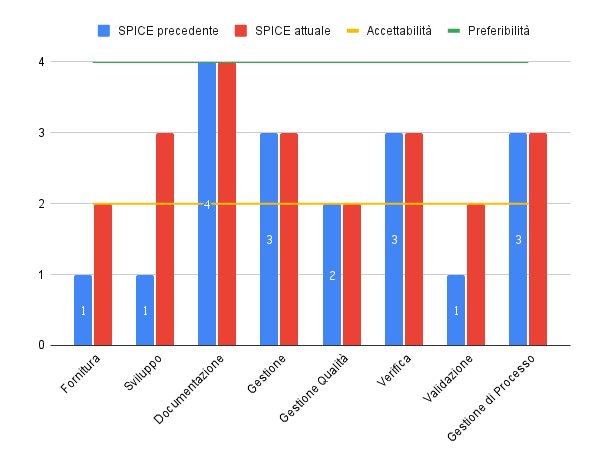
\includegraphics[scale = 0.6]{sezioni/Images/PB/SPICE.png}
	\caption{MPP5 - SPICE capability}
\end{figure}

\subsubsection{MPP6 - Requirements Stability Index}

\begin{figure}[H]
	\centering
	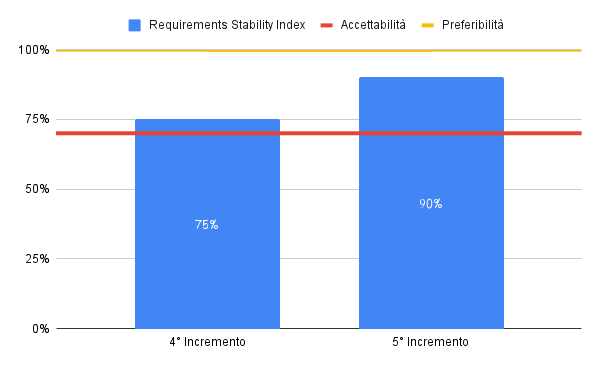
\includegraphics[scale = 0.6]{sezioni/Images/PB/RequirementsStabilityIndex.png}
	\caption{MPP6 - Requirements Stability Index}
\end{figure}

\subsubsection{MPR1 - Indice di Gulpease}

\begin{figure}[H]
	\centering
	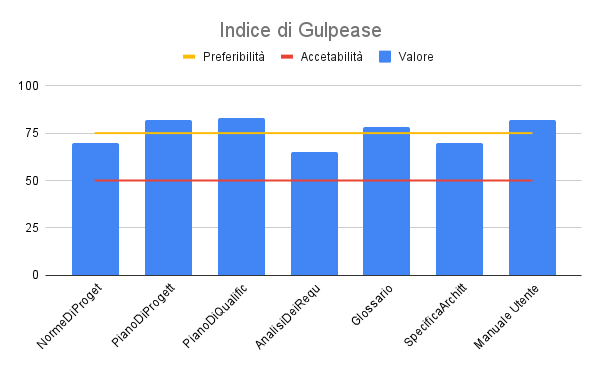
\includegraphics[scale = 0.6]{sezioni/Images/PB/GulpeaseGenerale.png}
	\caption{MPR1 - Indice di Gulpease delle norme di progetto}
\end{figure}

\subsubsection{MPR6 - Profondità gerarchia}
% Numero parametri per metodo
\subsubsection{MPR8 - Numero parametri per metodo}
% Code Coverage
%\subsubsection{MPR3 - Code Coverage}
% Percentuale requisiti obbligatori soddifatti
\subsubsection{MPR1 - Percentuale requisiti obbligatori soddisfatti}
% Complessità ciclomatica media
\subsubsection{MPR14 - Complessità ciclomatica media}
% Numero di bug ?
% Numero di Code smell ?
% Linee di commento per Linee di codice
\subsubsection{MPR10 - Linee commento per codice}
% Successo di test
\subsubsection{MPR16 - Percentuale test passati}
% Numero di vulnerabilità